\newpage
\section{Methodology}
\subsection{About the Dataset}


\subsubsection{Transcript Extraction and Annotation Process}

The ClaimBuster dataset was created by extracting sentences from transcripts of all U.S. presidential debates from 1960 to 2016. Initially, sentences spoken by the presidential candidates were identified using both automated parsing tools and manual verification to ensure accuracy. Sentences spoken by others, such as moderators or audience members, were excluded to maintain focus on the candidates' statements. Short sentences under five words were also removed to concentrate on more substantive content. This selection process resulted in a dataset of 23,533 sentences. \cite{claimbuster_arslan}. 

The following figures show an evolution of sentence volume and average sentence length in U.S. presidential debates over time. While the total number of sentences per debate has risen, the average sentence length per debate seems to have declined across the timeline. This observation aligns with the general shift in english language towards the usage of shorter sentences \cite{sentence_length_1}.

\begin{figure}[h]
    \centering
    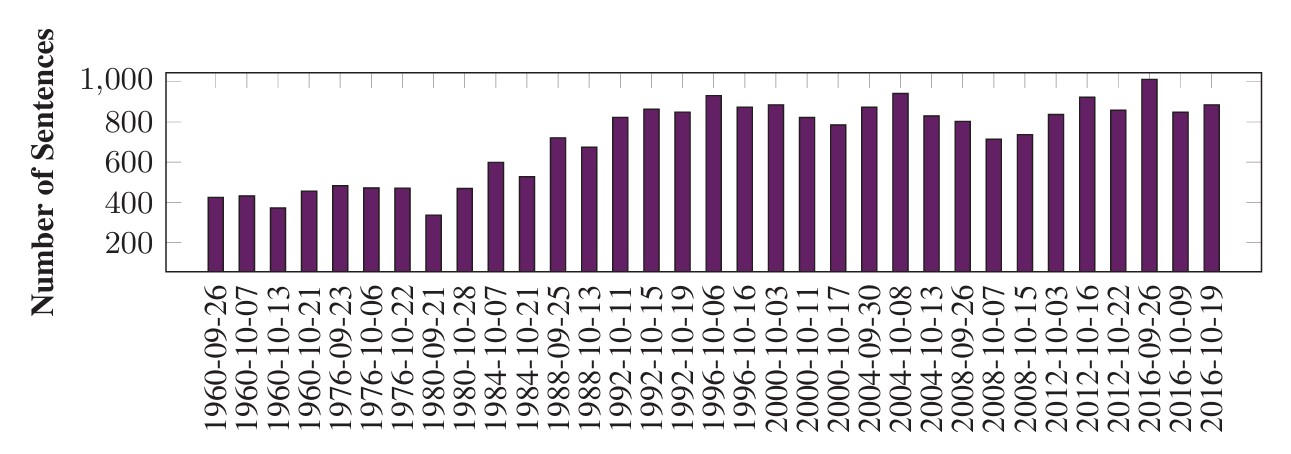
\includegraphics[width=1\textwidth]{assets/Claimbuster_Number_of_Sentences.jpg}
    \caption{Sentence distribution among presidential debates \cite{claimbuster_arslan}.}
    \label{fig:my_label}
\end{figure}

\begin{figure}[h]
    \centering
    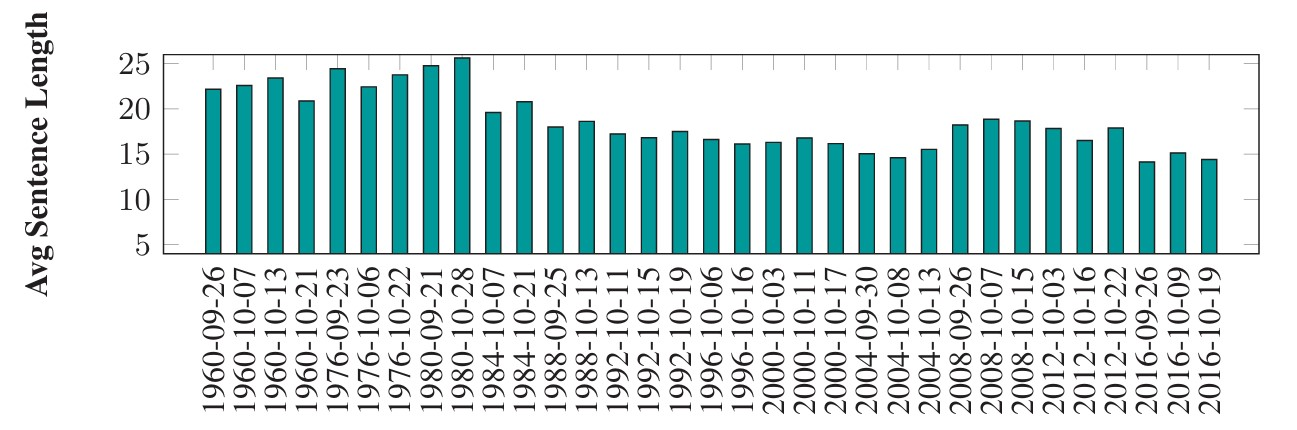
\includegraphics[width=1\textwidth]{assets/Claimbuster_Sentence_Length.jpg}
    \caption{Average sentence length in words per debate \cite{claimbuster_arslan}.}
    \label{fig:my_label}
\end{figure}

\subsubsection{Annotation Procedure}
The annotation process was an important part of developing the ClaimBuster dataset \cite{claimbuster_arslan}. The sentences were classified into one of three categories:

\glspl{nfs}: Sentences that did not contain verifiable claims.

\glspl{ufs}: Factual statements that were considered trivial or not significant enough to require verification.

\glspl{cfs}: Factual statements determined significant enough to require verification due to their potential impact on public discourse.

Figure 4 illustrates the distribution of these categories across all U.S. presidential debates from 1960 to 2016 from which the sentences were gathered. While there are some variations across the timeline, there is no discernible trend in the distribution of categories over time.

\begin{figure}[h]
    \centering
    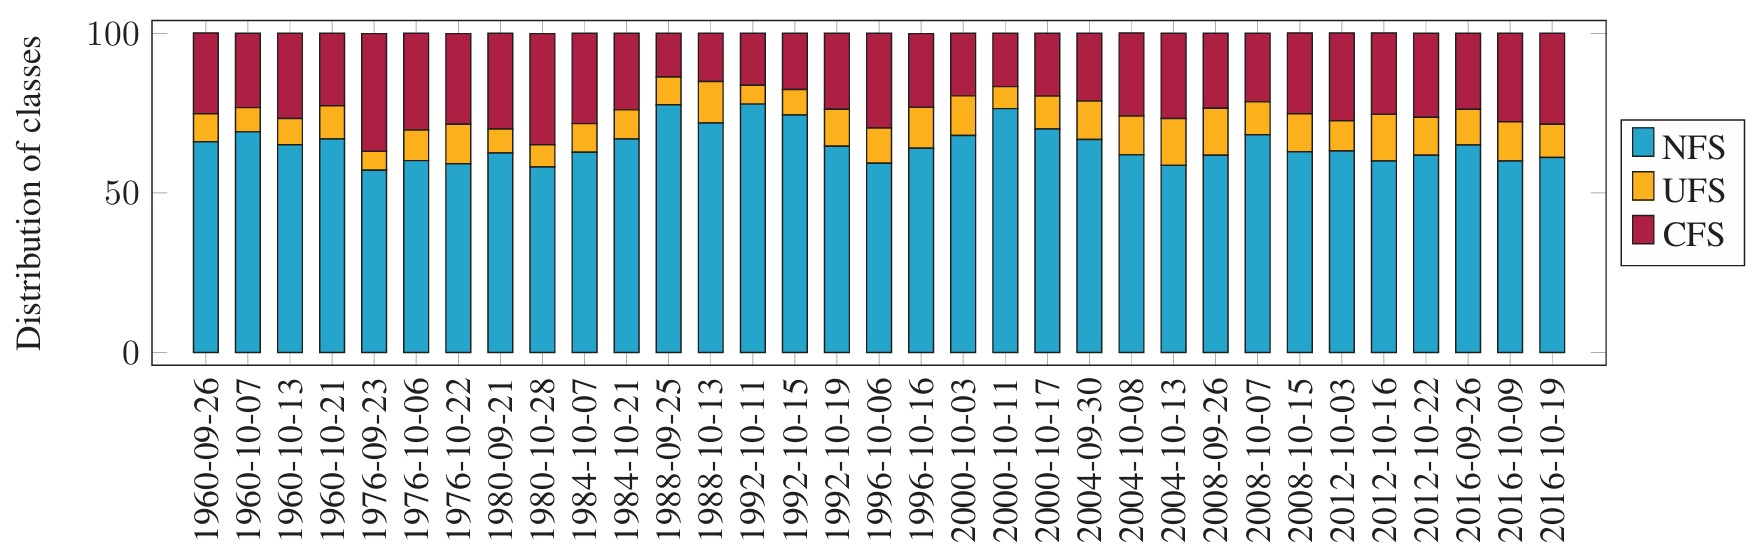
\includegraphics[width=1\textwidth]{assets/NFS_UFS_CFS.jpg}
    \caption{Category distribution per debate \cite{claimbuster_arslan}.}
    \label{fig:my_label}
\end{figure}

To ensure the objectivity and reliability of the annotations, each sentence was reviewed by multiple coders over a 26-month period. The coders were trained and provided with detailed guidelines to help them  categorize the sentences with improved accuracy. The involvement of multiple coders aimed to minimize individual biases and improve the consistency of the annotations \cite{claimbuster_arslan}.

\subsubsection{Quality Control Measures}
To maintain the targeted high accuracy of annotations, a subset of the sentences was used to create a 'ground-truth' dataset. This subset was annotated by a team of three expert reviewers. On average, every tenth sentence presented to the coders for annotation was from this 'ground truth' dataset. Based on these already labeled sentences, the accuracy of the predictions made by each coder was tested. With a point system that affected the money earned per annotated sentence, coders were penalized for low annotation accuracy but rewarded for high accuracy. Their performances on these control sentences were used to assess their overall reliability and accuracy in annotation \cite{claimbuster_arslan}.

\subsubsection{Ethical Considerations and Fairness}

In the paper, the coders are described demographically as primarily students, supplemented by some professors and journalists. They were invited to participate using flyers, social media, and direct emails. There is an argument to be made about potential biases existing, mainly because most participants were students. Their views and political leanings might have a general consensus that deviates from that of the general public. However, the method of invitation through flyers and social media—tools used across all demographic groups—suggests that there were participants from different fields of study and various backgrounds. Secondly, since their performance was observed and continuously evaluated through the point system, annotations made by biased coders were actively excluded from the final evaluation \cite{claimbuster_arslan}.


\subsection{Data Analysis}
\subsubsection{Data Analysis Overview}
In our initial analysis, we examined the number of samples in each of the three datasets and the ratio of positive to negative labels within them. The following figure illustrates the distribution of sample counts across the three datasets: the training set, the development set, and the development-test set.

\begin{figure}[h]
    \centering
    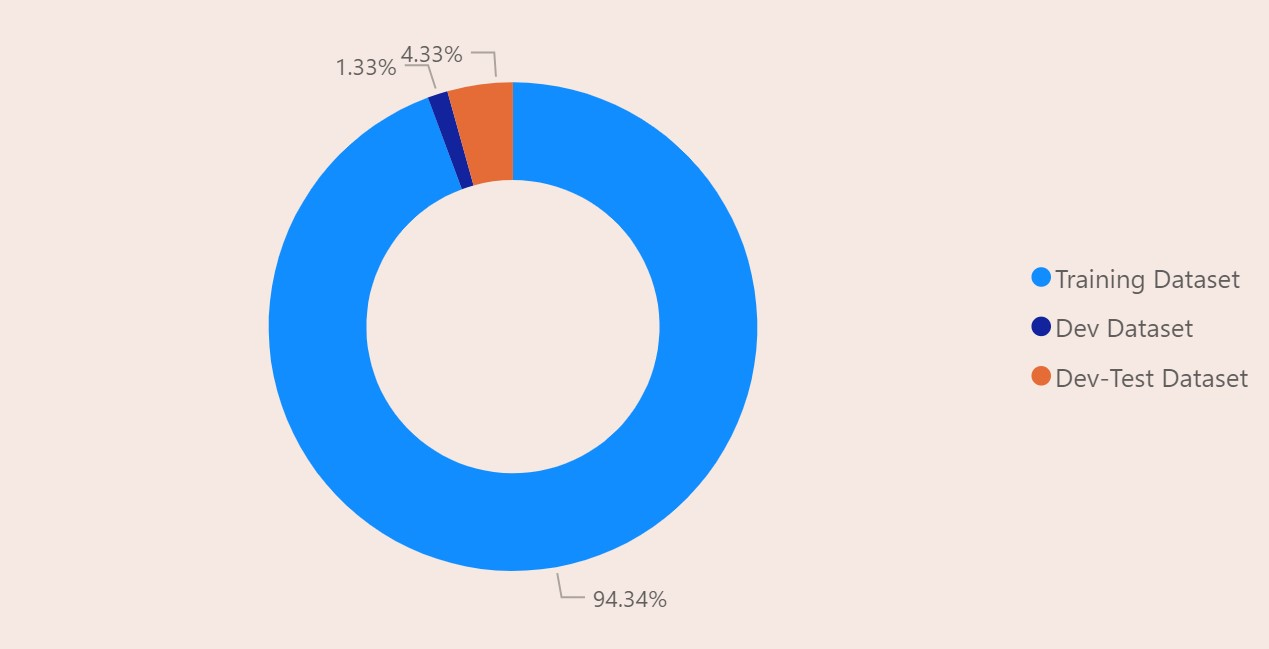
\includegraphics[width=0.9\textwidth]{assets/Sample_Distribution.jpg}
    \caption{Distribution of sample sizes across the three datasets}
    \label{fig:my_label}
\end{figure}

The training dataset is significantly larger, containing 22,501 samples, compared to the development dataset, which includes 1,032 samples used for validation during model training. The development-test dataset, used for model testing, is smaller yet, containing only 318 samples. This notable difference in sample sizes is primarily because the training data corresponds exactly to the crowd-sourced portion of the ClaimBuster dataset, while the development data matches the ground truth dataset described in the ClaimBuster paper \cite{claimbuster_arslan}. We assume this arrangement of data is intentional but remain open to the possibility of re-distributing or mixing the data if necessary. Moreover, the CheckThat! Lab categorized the \glspl{cfs} sentences from the ClaimBuster dataset as checkworthy and the \glspl{ufs} and \glspl{nfs} sentences as non-checkworthy.

\subsubsection{Text Sample Length Distribution Analysis}
Next, we analyzed the distribution of the lengths of the text samples, both overall and segmented by class. Figure~\ref{fig:my_length_barplot} depicts how the lengths of the samples are distributed.

\begin{figure}[h]
    \centering
    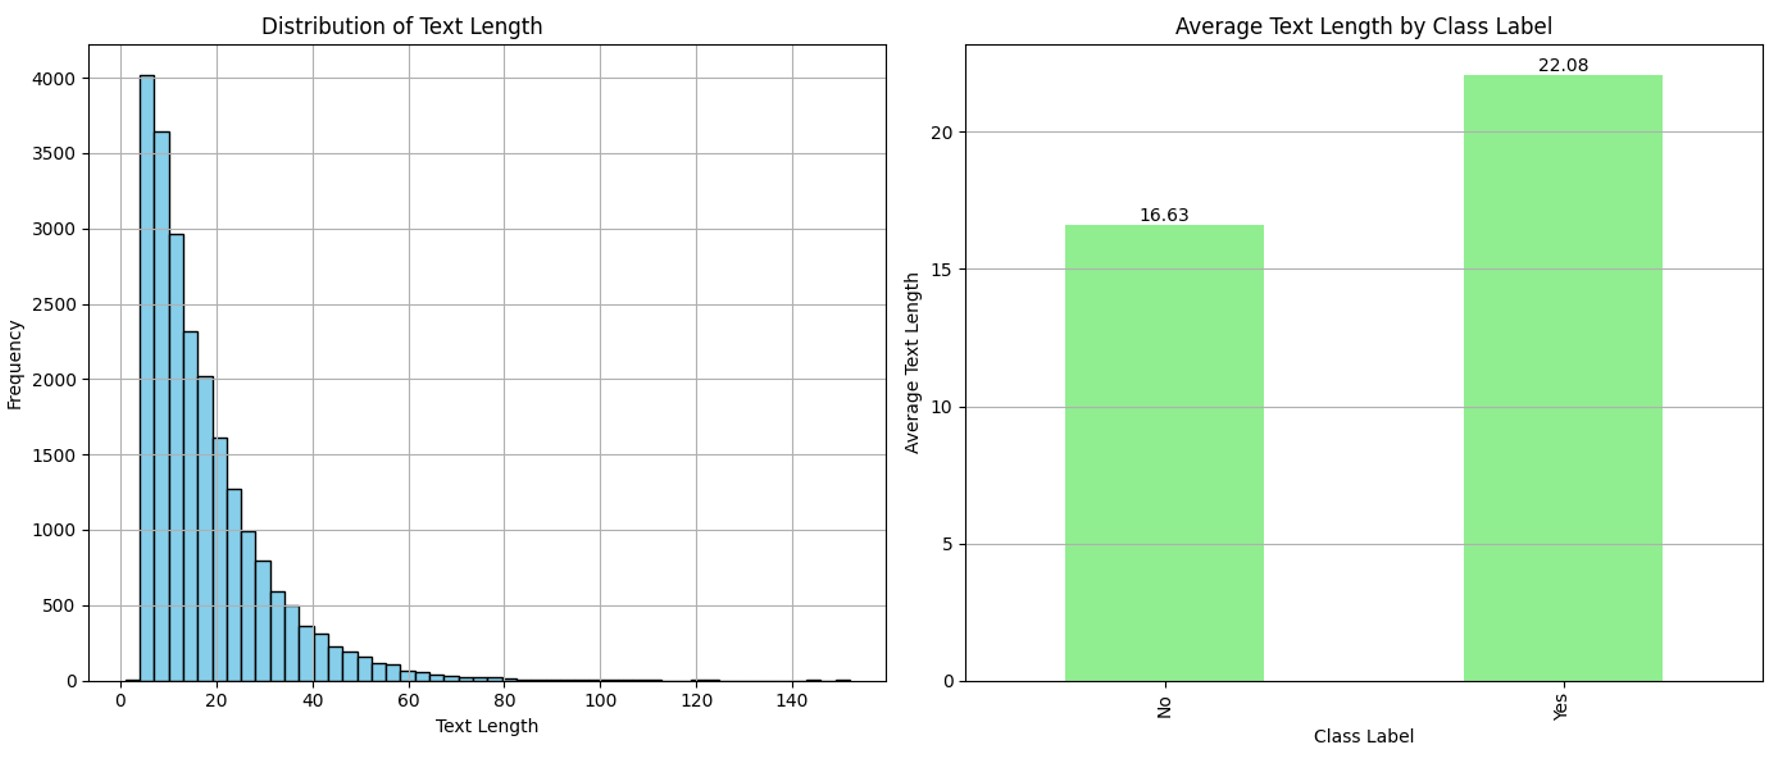
\includegraphics[width=1\textwidth]{assets/Text_Length_with_Barplot.jpg}
    \caption{Distribution of text lengths in the training dataset by class label}
    \label{fig:my_length_barplot}
\end{figure}


As expected, there are significantly more shorter samples than longer ones. However, it is noteworthy that the average length of positive samples is considerably longer than that of negative samples. According to the ClaimBuster paper, sentences shorter than five words were excluded from the dataset. Nonetheless, sentences containing only five words are less likely to include a claim due to their limited length, making it challenging to formulate a complete claim within such a brief context.

While this observation may seem trivial, it has important implications for the training of our deep learning models, which we will discuss in one of the following chapters. This insight into sample length distribution could influence model performance and the strategies we employ during the training process.


\subsubsection{Distribution of Class Labels} \label{dist_labels}
According to the paper, all statements from the debate transcripts spoken by political candidates were used, except for those under five words in length \cite{claimbuster_arslan}. This suggests that the assignment of check-worthy labels may be more random than intentional. Interestingly, as shown in the following figure, the ratio of negative to positive labels in both the training and development datasets is approximately 3:1. In contrast, the ratio in the test dataset markedly differs, at about 2:1 in favor of negative samples. This disparity suggests that the test sample may originate from a different source, which we could not identify.

\subsubsection{Statistical Text Analysis}
To better understand the thematic content of our training dataset, we started by determining the most common words based on the classification label of the text samples in which they appear, initially by simply counting their occurrences. The resulting graphic displays the words that appear most frequently in each of the two 'classes'.

\begin{figure}[h]
    \centering
    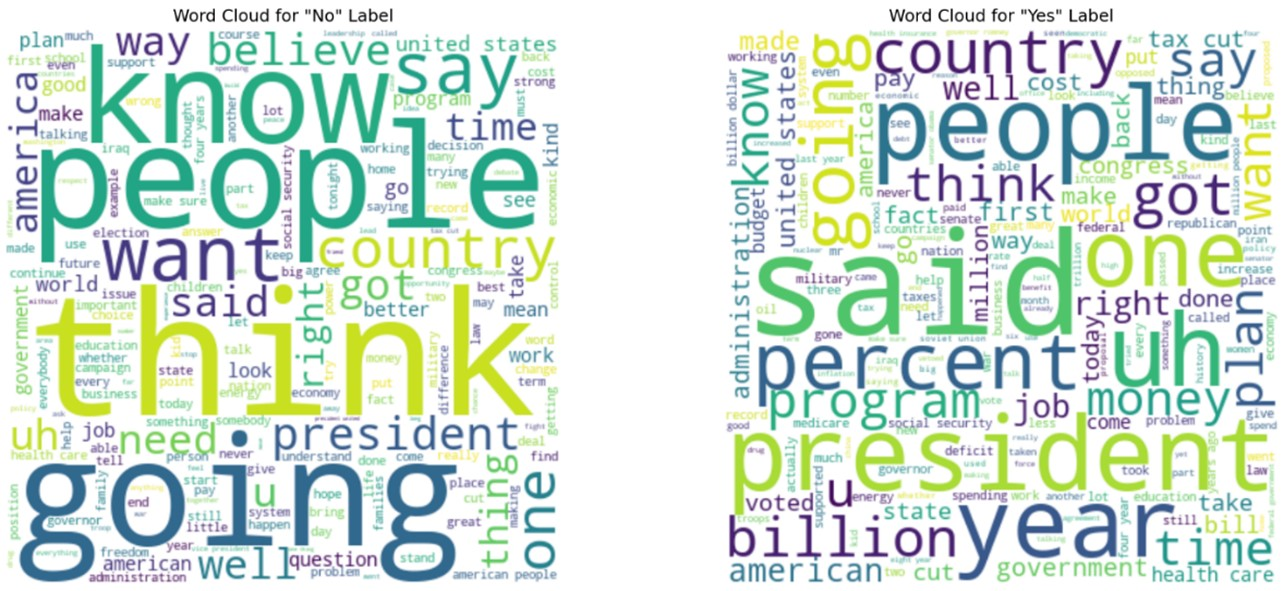
\includegraphics[width=1\textwidth]{assets/word_cloud.jpg}
    \caption{Most common words in the training dataset per class label}
    \label{fig:my_label}
\end{figure}

It is important to note that very short words, known as 'stop words', were excluded from this analysis because they often appear frequently but do not significantly alter the meaning of a sentence.

To further enhance this analysis, we conducted a \gls{tf-idf} analysis on the training dataset, considering both unigrams and bigrams. \gls{tf-idf} is a statistical measure used to evaluate how important a word is to a document within a collection of documents \cite{TF-IDF}. In this context, 'Term Frequency' refers to the raw count of a term in a document, which can be adjusted by the length of the document or by the raw frequency of the most frequently occurring word in the document. 'Inverse Document Frequency' measures how unique a word is across the entire dataset; it is calculated by dividing the total number of documents by the number of documents containing the term, and then taking the logarithm of that quotient. A word common across many documents will have a lower score, approaching 0, while rarer words will approach a higher value, near 1.

The product of these two metrics, the TF and the IDF, results in the \gls{tf-idf} score. A higher \gls{tf-idf} score indicates that a word is more relevant to a specific document within the dataset \cite{TF-IDF}.

Following the \gls{tf-idf} analysis, we trained a \glspl{svm} classifier model on this vectorized matrix from the training dataset to predict the labels of the development and test datasets. We utilized a LinearSVC with parameters set for balanced class weight and a fixed random state for reproducibility. To determine which terms most strongly influence the classifier's decisions towards positive or negative labels, we analyzed the coefficients of the n-grams. We sorted these coefficients by their values, identifying the most positive and the most negative coefficients. We then matched these coefficients to their corresponding n-gram indices within the model to pinpoint the specific n-grams associated with the most significant influences on the classifier's decisions. The following graphic shows the n-grams with the highest and lowest coefficients obtained from the \gls{svm} classifier.

\begin{figure}[h]
    \centering
    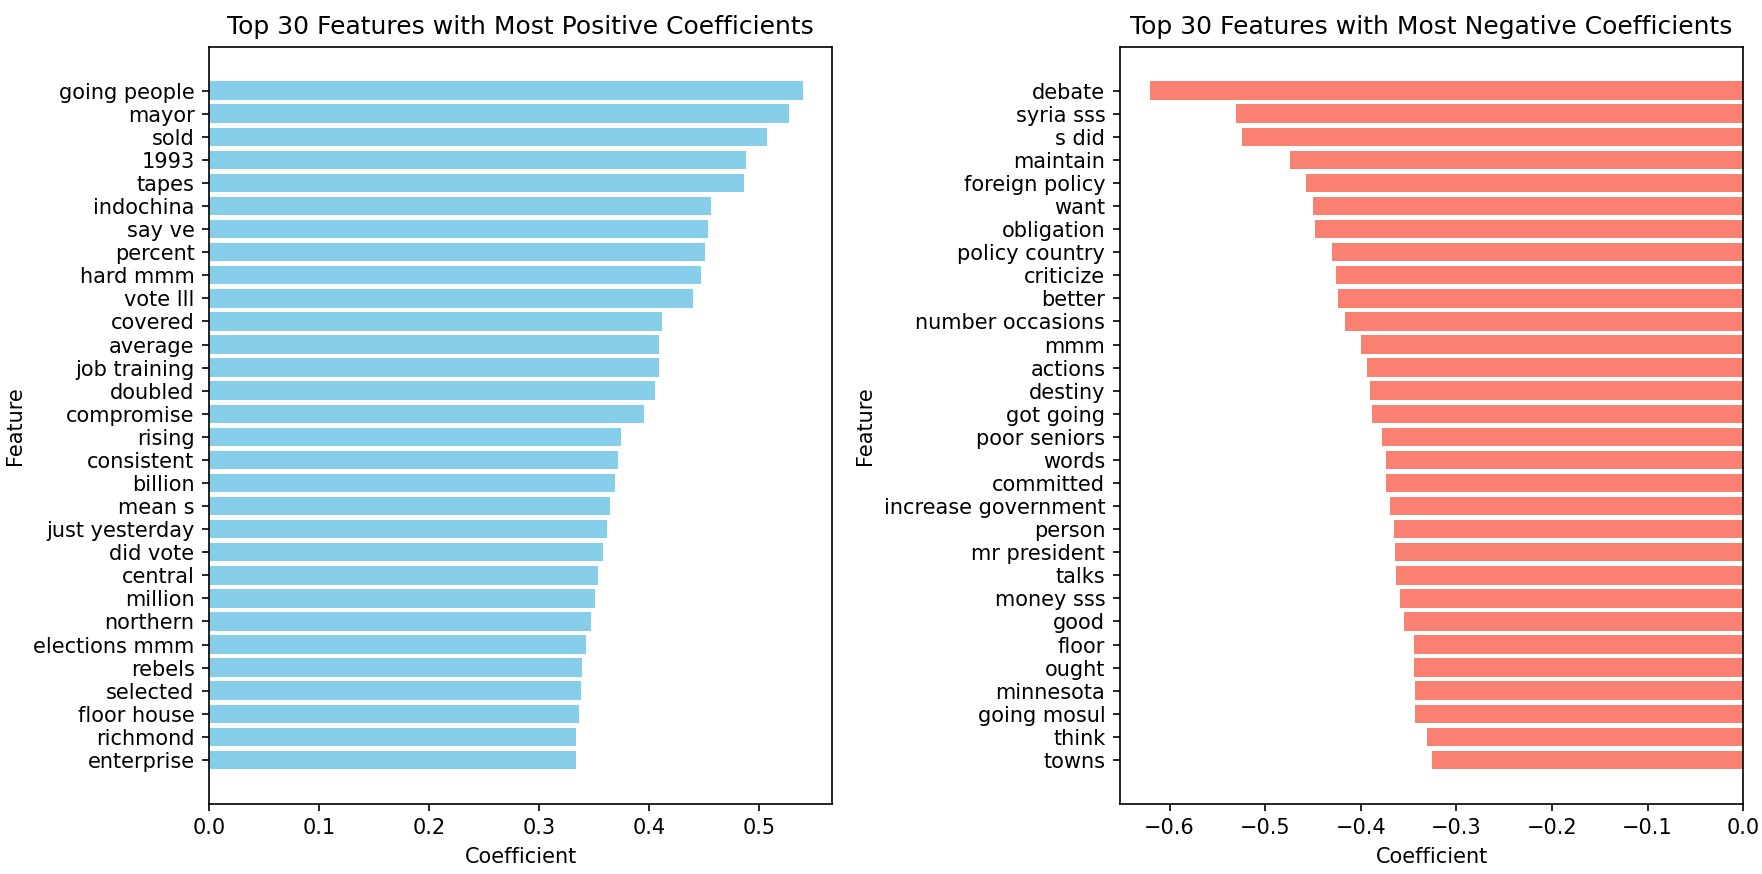
\includegraphics[width=1\textwidth]{assets/svm_coef.jpg}
    \caption{Influential n-grams in classification decisions of the svm model}
    \label{fig:my_label}
\end{figure}


\subsubsection{Results}

\newpage
\subsection{Fine-tuning} \label{fine-tuning}

Given the success of \glspl{plm} in text classification tasks \cite{textclass2021review}, we decided to adopt this approach for our classification task.
The first step was to select state-of-the-art \glspl{plm} and to fine-tune them with the original dataset described in \ref{}. To select the \glspl{plm}, we conducted thorough literature search using keywords such as 'Text classification', 'Transfer Learning in NLP', 'BERT-based Models'. Subsequently, we prioritized models that had demonstrated strong performance on \gls{nlu} benchmarks. Table \ref{tab:performance_plm}, adapted from \cite{he2021debertav3}, provides an overview of the performance of the models on the MNLI matched/mismatched (m/mm) \cite{mnli2018} and on the SQuAD v2.0 \cite{squad2018} development set.
Another criterion taken into account is the availability of the model on HuggingFace\footnote{\url{https://huggingface.co}.}. Hugging Face provides a convenient platform for accessing \glspl{plm}.
Based on these criteria, we selected the following \glspl{plm} for the fine-tuning process: RoBERTa\textsubscript{base}\footnote{\url{https://huggingface.co/FacebookAI/roberta-base}.} \cite{roberta2019}, XLNet\textsubscript{base}\footnote{\url{https://huggingface.co/xlnet/xlnet-base-cased}.} \cite{xlnet2019}, ELECTRA\textsubscript{base}\footnote{\url{https://huggingface.co/google/electra-base-discriminator}.} \cite{electra2020}, DeBERTaV3\textsubscript{base}\footnote{\url{https://huggingface.co/microsoft/deberta-v3-base}.} \cite{he2021debertav3}.

\begin{table}[h]
    \centering
    \begin{tabular}{l|cc}
    \hline
         \textbf{Model}&MNLI-m/mm(ACC)&SQuAD 2.0(F1/EM)\\
    \hline
         RoBERTa\textsubscript{base}&0.876/-&0.837/0.805\\
         XLNet\textsubscript{base}&0.868/-&-/0.802\\
         ELECTRA\textsubscript{base}&0.888/-&-/0.805\\
         DeBERTa\textsubscript{base}&0.888/0.885&0.862/0.831\\
         DeBERTaV3\textsubscript{base}&0.906/0.907&0.884/0.854\\
    \hline
    \end{tabular}
    \caption{Performance of state-of-the-art \glspl{plm}. Adapted from \cite{he2021debertav3}}
    \label{tab:performance_plm}
\end{table}

All the selected models are based on BERT, which stands for Bidirectional Encoder Representations from Transformers. BERT is a language representation model. It was pretrained using two unsupervised tasks: \gls{mlm} and \gls{nsp}. In \gls{mlm} 15\% of the words in the sentence are masked with a [MASK] token and the model is trained with the objective to predict those masked words based on their left and right context. \gls{mlm} enables the language representation to be conditioned on both the left and right context. Through \gls{nsp}, the model learns to predict whether a given sentence B follows a given sentence A, which helps the model to understand sentence relationships. \cite{bert2019}. However, all the selected models omit the \gls{nsp} task stating that the \gls{nsp} task does not significantly improve model performance \cite{roberta2019, xlnet2019, electra2020}.

RoBERTa improves BERT by optimizing the pretraining procedure. Specifically, it removes the \gls{nsp} task and uses dynamic masking instead of static masking. Additionally, RoBERTa uses larger training times, larger batches and approximately ten times more training data. Specifically, it was trained on a combination of BookCorpus, English Wikipedia, CC-News, OpenWebText, and Stories, totalling over 160 GB of data \cite{roberta2019}.

XLNet is an autoregressive pretraining model that addresses some limitations of BERT by using a permutation-based training objective, allowing it to model bidirectional context without the need for masking. In this permutation-based training, the model considers all possible arrangements of the words in the sentence, not just the original order \cite{xlnet2019}. XLNet\textsubscript{base} was pretrained on BooksCorpus, English Wikipedia, Giga5, ClueWeb 2012-B and Common Crawl, which combined give over 158 GB of data \cite{xlnet_github, xlnet2019}.

ELECTRA is a discriminator model that builds upon the bidirectional modeling ideas of BERT but replaces the \gls{mlm} task with a more compute-efficient task called \gls{rtd}. In \gls{rtd}, instead of masking the words, they are replaced with plausible alternatives generated by a small generator network. ELECTRA is then trained to distinguish between original and replaced tokens. This approach is more compute-efficient because the model learns from the entire input sentence rather than just the smaller masked subset \cite{electra2020}. The Base version of ELECTRA is pretrained on the same dataset as XLNet \cite{electra_github, electra2020}.

DeBERTa improves upon BERT by introducing two main techniques: disentangled attention and an enhanced mask decoder. In disentangled attention, each word is represented by two vectors, one for content and one for position. This allows the model to better capture the relationships between words and their positions in a sentence. The enhanced mask decoder improves the model’s ability to reconstruct masked tokens by using a more sophisticated decoder \cite{he2021debertav3}. The latest version of DeBERTa, DeBERTaV3, incorporates the \gls{rtd} task from ELECTRA, replacing the \gls{mlm} task. DeBERTaV3 was pretrained using the same data as RoBERTa \cite{he2021debertav3}.

To ensure robust evaluation, multiple fine-tuning runs for each model were conducted. This approach helps to mitigate the impact of randomness in training and provides a more reliable estimate of the models' performance.
The training set was used to fine-tune the models, the development set was used to evaluate performance during training and to select the best checkpoint, and the development-test set was used to evaluate the final performance of each model on unseen data.
The hyper-parameters utilized are consistent with those employed by von Däniken et al. \cite{vondaniken2023} in their fine-tuning of the \textit{electra-clf} model for the CheckThat! Lab 2023. The training hyper-parameters are detailed in Table \ref{tab:hyperparam}. Additionally, we introduced a checkpoint saving strategy every 400 steps during training. At the end of training, the checkpoint with the highest F1 score on the validation set was selected as the final model, since the official evaluation metric for Task 1 of the CheckThat! Lab 2024 is the F1 score over the positive class.  


\begin{table}[h]
    \centering
    \begin{tabular}{l|c}
    \hline
         \textbf{Hyper-parameter}&Value\\
    \hline
         Epochs&10\\
         Batch Size&16\\
         Optimizer&AdamW\cite {adam_w}\\
         Learning Rate&5e-5\\
         Weight Decay&0.01\\
         Warmup Steps&500\\
         Learning Rate Decay&Linear\\
    \hline
    \end{tabular}
    \caption{Hyper-parameters for fine-tuning the \glspl{plm}. Adapted from \cite{}}
    \label{tab:hyperparam}
\end{table}

\paragraph{Results}
Table \ref{tab:finetune_scores} presents the scores of each fine-tuned model on the development set and on the development-test set. For each model, we report the mean and standard deviation of the accuracy, precision, recall, and F1 score over multiple runs. 

\begin{table}[h]
    \centering
    \begin{tabular}{l|c|c|c|c}
    \hline
         \textbf{Model} & F1 Score & Accuracy & Precision & Recall \\
    \hline
    \hline
        \multicolumn{5}{l}{\textit{Scores on development set}}\\
        RoBERTa\textsubscript{base}& 0.944 $\pm$ 0.010 & 0.974 $\pm$ 0.005 & 0.932 $\pm$ 0.041 & 0.958 $\pm$ 0.024\\
        XLNet\textsubscript{base} & 0.939 $\pm$ 0.004 & 0.971 $\pm$ 0.001 & 0.930 $\pm$ 0.015& 0.948 $\pm$ 0.015\\
        ELECTRA\textsubscript{base} & 0.941 $\pm$ 0.011 & 0.973 $\pm$ 0.005 & 0.939 $\pm$ 0.006& 0.942 $\pm$ 0.017\\
        DeBERTaV3\textsubscript{base} & 0.947 $\pm$ 0.004 & 0.975 $\pm$ 0.002 & 0.933 $\pm$ 0.003& 0.962 $\pm$ 0.006\\
    \hline
        \multicolumn{5}{l}{\textit{Scores on development-test set}}\\
         RoBERTa\textsubscript{base}& 0.818 $\pm$ 0.028 & 0.890 $\pm$ 0.009 & 0.934 $\pm$ 0.056 & 0.732 $\pm$ 0.079 \\
         XLNet\textsubscript{base} & 0.821 $\pm$ 0.026 & 0.892 $\pm$ 0.016 & 0.930 $\pm$ 0.026& 0.732 $\pm$ 0.026 \\
         ELECTRA\textsubscript{base} & 0.832 $\pm$ 0.017 & 0.899 $\pm$ 0.011 & 0.951 $\pm$ 0.034 & 0.741 $\pm$ 0.025 \\
         DeBERTaV3\textsubscript{base} & 0.849 $\pm$ 0.030 & 0.909 $\pm$ 0.016 & 0.965 $\pm$ 0.009 & 0.759 $\pm$ 0.052 \\
    \hline
    \end{tabular}
    \caption{Performance metrics of fine-tuned models on development set and on development-test set}
    \label{tab:finetune_scores}
\end{table}

On the development set, DeBERTaV3 achieved the highest mean F1 Score of 0.947, closely followed by RoBERTa with a mean F1 score of 0.944. Overall, all models achieved high scores on the performance metrics. The standard deviations were relatively low across all models, indicating consistent performance during multiple runs.

For the development-test set, DeBERTaV3 again showed the best performance with a mean F1 score of 0.849. ELECTRA followed with a mean F1 score of 0.832. The standard deviations were slightly larger on the development-test set, indicating more variability in performance across different runs.

When comparing the performance across the two sets, there is a noticeable drop in the F1 score when the models are evaluated on the development-test set. The recall metric is particularly affected, e.g., for the DeBERTaV3 model, recall drops by 21.1\%. Precision, on the other hand, remains stable or even improves in some cases in the development-test set.

Figure \ref{fig:loss_curve} illustrates the training and evaluation loss for the DeBERTaV3 and RoBERTa models during the fine-tuning process. The training loss starts high, around 0.6, and drops sharply within the first 2000 training steps, reaching approximately 0.2. It continues to decrease but at a slower rate, dropping below 0.1 with minor fluctuations around 6000 steps. After 8000 steps, the training loss converges to 0. On the other hand, the evaluation loss starts around 0.3 and stabilizes around 0.1 in the first 1000 steps. After 4000 steps, it starts to gradually increase, reaching 0.2 at around 7000-step mark and approximately maintaining this loss until the end of the training. Most of the other models show a similar course. In the case of the RoBERTa model, the training loss decreases more slowly compared to the other models. However, the evaluation loss for RoBERTa remains slightly below that of the other models after the 6000-step mark.

\begin{figure}[H]
    \centering
    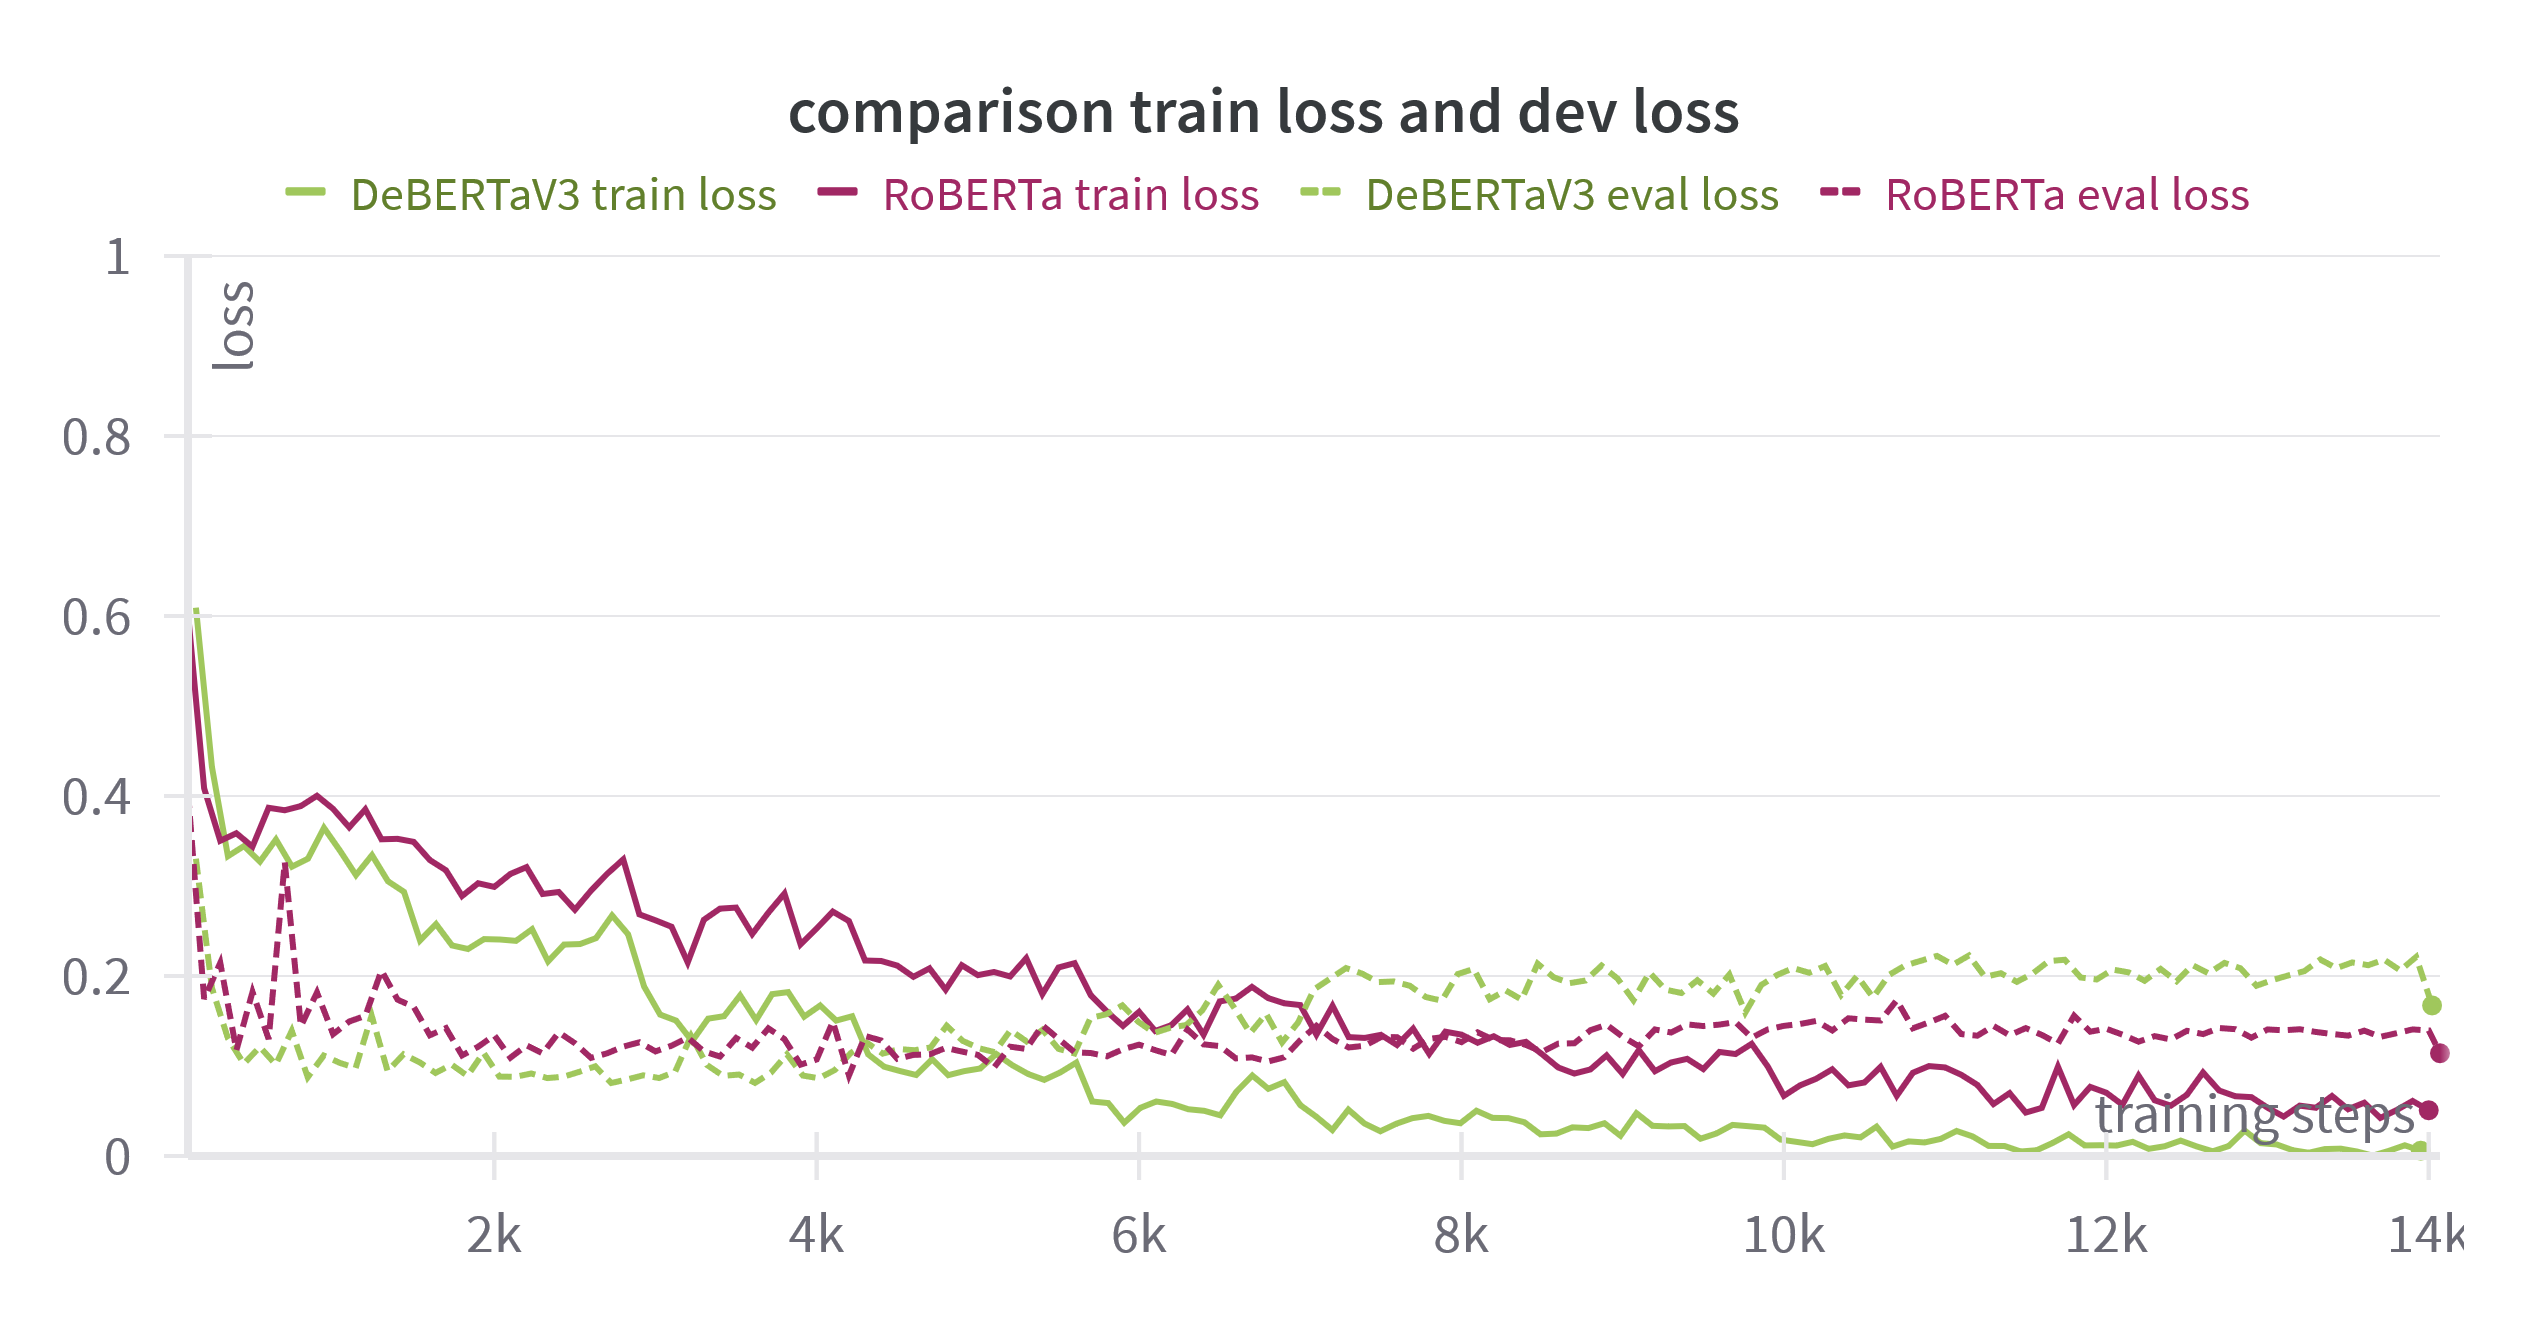
\includegraphics[width=1\linewidth]{assets/deberta and roberta loss curves.png}
    \caption{Loss curves on the training set and development set for the DeBERTaV3 and RoBERTa models. To maintain clarity in the plot, the loss curves for the other models, which exhibit similar patterns to the DeBERTaV3 curves, are omitted.}
    \label{fig:loss_curve}
\end{figure}

%TODO maybe write that the checkpoint loading strategy with the best f1 score sometimes loaded models where the evaluation loss was in the potential overfitting area. We thought this could load a checkpoint that does not generalize well to unseen data, so we tried to use the eval loss as the best metric for the saving strategy. This did not improve the performance on the development-test set so we kept the f1 score. Then we also tried early stopping with the f1 score and patience once 5 and once 10 (eval_steps = 100) to prevent possible overfitting, but this also did not improve performance and is some case was much worse.

%TODO explain probability calibration. Precision-recall curve. Threshold finetuning to find a better trade off between precision/recall.

\subsubsection{Discussion}
The DeBERTaV3 model achieved the highest F1 scores on both sets suggesting that it is the most effective model for this task among those tested. This is reasonable since DeBERTaV3, as seen on Section \ref{fine-tuning}, further enhanced their model based on the successful \gls{rtd} technique from ELECTRA, and outperforms the other models on \gls{nlu} benchmarks.

The observed drop in performance on the development-test set suggests that this set contains more challenging or diverse examples. In Section \ref{dist_labels} we describe that:
\begin{enumerate}
    \item The origin of the development-test set is unknown, and it is unclear whether the same methods used for labeling the training and development sets were applied to the development-test samples.
    \item The class label distribution differs between the development-test set and the other sets.
\end{enumerate}
These factors could explain the significant performance gap between the development and development-test sets. Given the lack of information to address the first point, we decided to focus on the second point.

The rapid decrease in both training and evaluation loss during the initial phase of training indicates effective early learning, with the model quickly capturing the primary patterns in the data. The continuing decrease in training loss and the slight increase in evaluation loss hint at potential overfitting. This scenario, where the model performs better on training data but worse on unseen data, should be prevented through the checkpoint loading strategy described in Section \ref{fine-tuning}.

\newpage
\subsection{Data Manipulation: Analyzing Effects on Model Performance}
To further enhance the F1 score and optimize our model's predictive accuracy, we explored strategic modifications to the dataset configuration. Our primary objective was to enable the model to learn more effectively from the training data.

\subsubsection{Sample Redistribution across Datasets}
Our initial approach involved shuffling the three datasets—training, development, and development-test—so that all samples were evenly distributed among them. The rationale behind this strategy was inspired by a paper concerning the ClaimBuster dataset, which suggested that the development dataset arguably possesses more reliable class labels due to its 'ground truth' data \cite{claimbuster_arslan}.

By redistributing the samples, our intention was to introduce a higher proportion of reliable data into the training set, potentially enhancing overall model performance. This shuffling was performed using a random algorithm, ensuring that the distribution of class labels across each dataset remained random. However, we maintained the original size of each dataset split (22,501 in the training dataset, 1,032 in the development dataset, and 318 in the test dataset.

To evaluate the impact of this redistribution, we trained three of our best-performing models on the shuffled dataset: Google’s Electra Base, Microsoft’s DeBERTa v3 Base, and XLNet Base.

\paragraph{Results}
Contrary to our expectations, all three models demonstrated significantly reduced performance on the shuffled datasets compared to their performance on the original dataset configuration. Table~\ref{tab:shuffle_scores} shows the mean and standard deviation of the F1 score, accuracy, precision and recall for each model across multiple runs, differentiating between training on the shuffled and original datasets. 

\begin{table}[h]
    \centering
    \begin{tabular}{l|c|c|c|c}
    \hline
         \textbf{Model} & F1 Score & Accuracy & Precision & Recall \\
    \hline
    \hline
        \multicolumn{5}{l}{\textit{Scores on development-test set of models trained on shuffled training set}}\\
        XLNet\textsubscript{shuffled} & 0.694 $\pm$ 0.016 & 0.862 $\pm$ 0.002 & 0.714 $\pm$ 0.015 & 0.676 $\pm$ 0.018\\
        ELECTRA\textsubscript{shuffled} & 0.702 $\pm$ 0.028 & 0.859 $\pm$ 0.014 & 0.689 $\pm$ 0.017 & 0.716 $\pm$ 0.032\\
        DeBERTaV3\textsubscript{shuffled} & 0.698 $\pm$ 0.005 & 0.859 $\pm$ 0.003 & 0.693 $\pm$ 0.004 & 0.703 $\pm$ 0.007\\
    \hline
        \multicolumn{5}{l}{\textit{Scores on development-test set of models trained on original training set}}\\
         XLNet\textsubscript{base} & 0.821 $\pm$ 0.026 & 0.892 $\pm$ 0.016 & 0.930 $\pm$ 0.026 & 0.732 $\pm$ 0.026\\
         ELECTRA\textsubscript{base} & 0.832 $\pm$ 0.017 & 0.899 $\pm$ 0.011 & 0.951 $\pm$ 0.034 & 0.741 $\pm$ 0.025\\
         DeBERTaV3\textsubscript{base} & 0.849 $\pm$ 0.030 & 0.909 $\pm$ 0.016 & 0.965 $\pm$ 0.009 & 0.759 $\pm$ 0.052\\
    \hline
    \end{tabular}
    \caption{Comparing performance metrics of fine-tuned models trained on shuffled and original training sets}
    \label{tab:shuffle_scores}
\end{table}


As illustrated in Table~\ref{tab:shuffle_scores}, the average F1 scores for these models were approximately 0.7, indicating a strong decline in predictive efficacy.

\subsubsection{Data Augmentation with GPT}

Data augmentation is a widely adopted method for generating additional training data, which is particularly advantageous when applying deep learning models \cite{data_aug_shorten2021text}. This technique involves artificially expanding the dataset by creating modified versions of existing data or generating entirely new data points. In the context of text data, this can involve altering or generating text sequences to provide a richer and more diverse training set for machine learning models \cite{data_aug_abulaish2019text}.

Inspired by methodologies described in research conducted by members of the Check That Lab \cite{ct_23_033_gptaugmenation}, we incorporated data augmentation into our approach. For the generation of new samples, we relied on GPT-3.5, a model from OpenAI’s Generative Pre-trained Transformer series. GPT models have demonstrated exceptional capabilities in generating coherent and contextually relevant text. \cite{data_aug_gpt_brown2020language}. Additionally, they offer an optimal balance between performance and cost-effectiveness, which was a crucial factor given the volume of data we intended to generate.

The process was executed as follows: We established a connection to GPT-3.5 via the OpenAI API, which allowed for full automation of the data generation process, avoiding the need for manual input through a chat interface. Initially, we provided the model with prompts containing five samples from our training dataset. Each prompt (refer to figure) instructed GPT-3.5 to autonomously generate ten additional, content-wise novel samples, along with determining the classification label ('Yes' or 'No'). Furthermore, it was specified that the text samples pertained to political debates and that the class label should be assigned based on whether the general public might consider the content in the text sample to contain a claim potentially involving misinformation, thereby making it ‘checkworthy’.

Through this automated, iterative process, we generated 22,501 new samples. These were subsequently integrated with the original training text samples, resulting in a far larger dataset which now contains 45,002 samples. 

\begin{table}[h]
    \centering
    \begin{tabular}{l|c|c|c|c}
    \hline
         \textbf{Model} & F1 Score & Accuracy & Precision & Recall \\
    \hline
    \hline
        \multicolumn{5}{l}{\textit{Scores on development-test set of Electra model trained on partly augmented training set}}\\
        ELECTRA\textsubscript{augm} & 0.819 $\pm$ 0.028 & 0.893 $\pm$ 0.014 & 0.963 $\pm$ 0.017 & 0.713 $\pm$ 0.032\\
    \hline
        \multicolumn{5}{l}{\textit{Scores on development-test set of Electra model trained on original training set}}\\
         ELECTRA\textsubscript{base} & 0.832 $\pm$ 0.017 & 0.899 $\pm$ 0.011 & 0.951 $\pm$ 0.034 & 0.741 $\pm$ 0.025\\
    \hline
    \end{tabular}
    \caption{Comparing performance metrics of Electra model trained on the partly augmented and original training sets}
    \label{tab:aug_scores}
\end{table}

\subsubsection{Filtering}

The creators of the ClaimBuster dataset implemented a method to refine their training dataset by selectively reducing its size. This refinement involved removing some samples that, based on evaluations of label assignment accuracy, had received less reliable class labels compared to others. Specifically, the text samples in the dataset '3xNCS.json' were compiled from the \textit{groundtruth} and \textit{crowdsourced} datasets using stricter criteria for label assignment. This was done to enhance the quality of the training data, which is expected to contribute to the development of more accurate models \cite{meng2020gradientbased}. In this study, the dataset maintains a strict ratio of sentences between these two classes, which is reflected in the file name (3x).

According to the authors, this method of filtering the dataset can aid in the training of deep learning models, leading to improved classification scores. This enhancement in model performance through the use of refined training datasets has also been demonstrated in the winning paper of the Check That! Labs 2023, Task 1b \cite{ct_23_040_filtering}. Furthermore, it is well-documented in the literature that pre-trained deep learning models can achieve high scores even with smaller training datasets, an insight that has long been recognized in the field of deep learning \cite{kaplan2020scaling}.

These observations on dataset refinement demonstrate the importance of data quality over quantity in the training of effective deep learning models, particularly in applications requiring the detection and classification of factual information.

\subsubsection{Quantile-Based Text Length Segmentation}
In our previous analysis of the datasets, a potential correlation was identified between the length of text samples and their classification labels ('Yes' and 'No'). Preliminary data suggested that samples labeled 'Yes' often consisted of longer text sequences. Based on these insights, we hypothesized that integrating text length into our training strategy could potentially enhance the performance of our predictive models.


\begin{figure}[h]
    \centering
    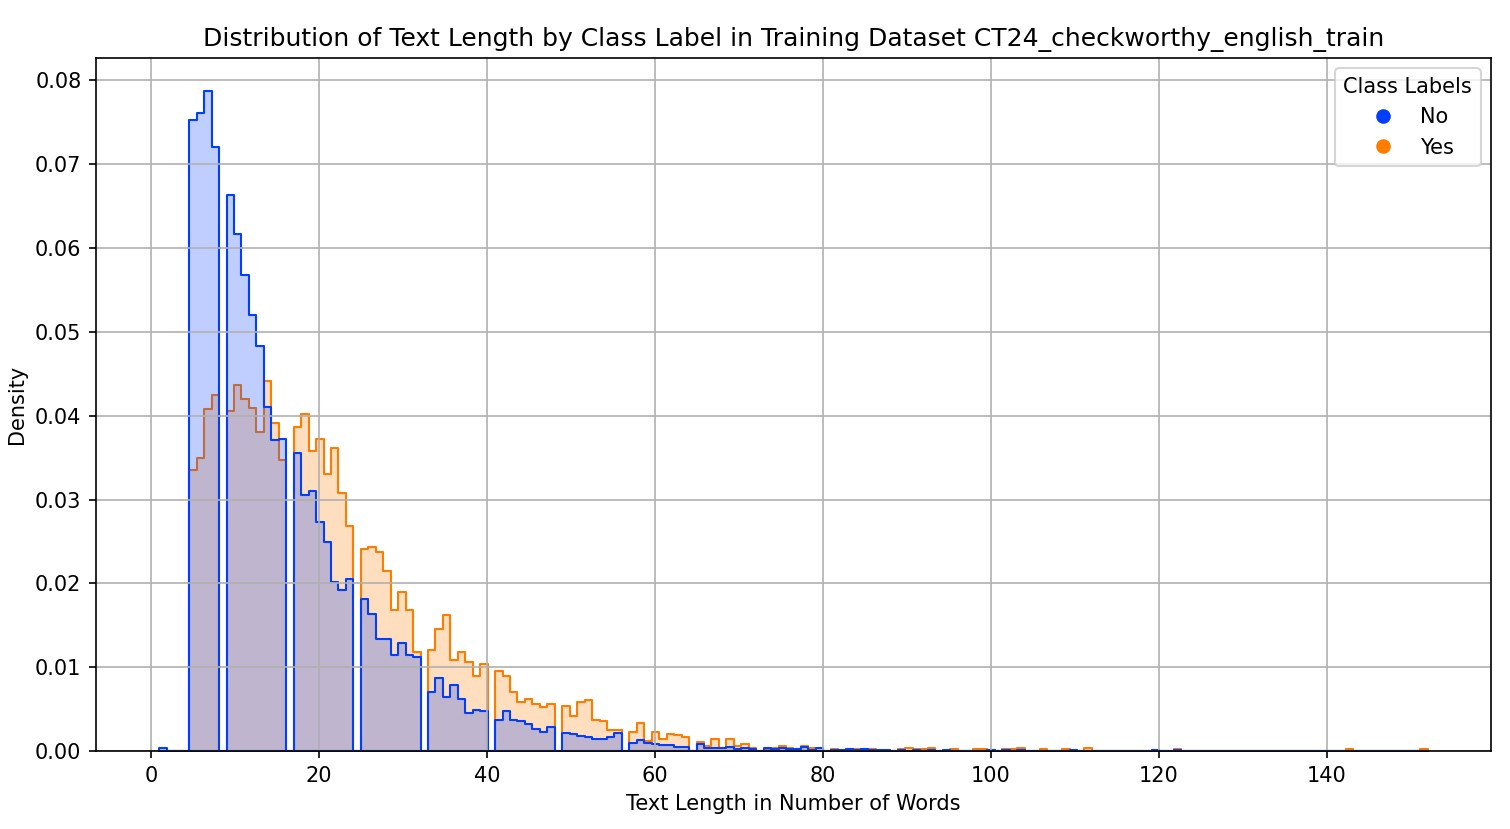
\includegraphics[width=1\textwidth]{assets/Text_Length.jpg}
    \caption{Distribution of text length in the training dataset by class label}
    \label{fig:my_label}
\end{figure}
To systematically incorporate text length into our model training, we adopted a method of classifying samples into three distinct categories based on their length. Each text sample was appended with a specific label indicating its length category. This categorization was implemented by defining quantiles based on the distribution of text lengths within the training data. The shortest third of samples received the label 'sss', the next shortest third 'mmm', and the longest third 'lll'.

These quantiles were determined using the training dataset but were then consistently applied to the development and development-test datasets using the same threshold values. This approach ensured uniformity in how text lengths were categorized across all datasets.

We applied this quantile-based segmentation to both the original and filtered datasets, subsequently training the Microsoft DeBERTa v3 base model with these modified datasets. This step was undertaken to evaluate whether the explicit consideration of text length could yield improvements in model performance, as measured by the F1 score.

\paragraph{Results}
The F1 scores obtained from models trained on these length-segmented datasets however, they did not significantly surpass the scores achieved prior to the implementation of this strategy. The accompanying graphic illustrates these findings, offering a visual representation of the comparative performance metrics.

\newpage
\subsection{Ensemble}
\subsubsection{Results}